%! TeX program = xelatex
\documentclass{beamer}

%% PACKAGES %%

% Macro making packages
\usepackage{xparse}
\usepackage{xpatch}
\usepackage{tokcycle}

% Standalone compilation
\usepackage[obeyclassoptions,mode=tex]{standalone}

% Math typesetting 
\usepackage{amsmath}
\usepackage{amsthm}
\usepackage{thmtools}
\usepackage{upgreek}
\usepackage{amssymb}
\usepackage{stmaryrd}

% References and knowledge management
\usepackage{hyperref}
\usepackage[capitalise,noabbrev,nameinlink]{cleveref}
\usepackage[electronic,hyperref,xcolor,cleveref]{knowledge}
\knowledgeconfigure{notion}

% BIBTEX / BIBLATEX
\usepackage[
	%style=numeric-comp,
    %citestyle=authortitle-icomp,
	citestyle=numeric-comp,
	%bibstyle=authoryear,
	bibstyle=numeric,
	%sorting=none,
    sorting=nyt,
	%sortcites=true,
	%autocite=footnote,
    maxnames=99,
    %backend=biber, % Compile the bibliography with biber
    backend=bibtex,
    %refsegment=chapter, % split references ?
	hyperref=true,
	backref=true,
	citecounter=true,
	pagetracker=true,
	citetracker=true,
	ibidtracker=context,
	autopunct=true,
	autocite=plain,
    doi=true,
]{biblatex}

% Table typesetting
\usepackage{booktabs}
\usepackage{varwidth}

% Proofs typesetting
\usepackage{bussproofs}

% Drawing
\usepackage{tikz}
\usetikzlibrary{backgrounds}
\usetikzlibrary{shapes.geometric}
\usetikzlibrary{positioning}
\usetikzlibrary{automata}
\usetikzlibrary{tikzmark}
\usetikzlibrary{patterns}
\usetikzlibrary{arrows}
\usepackage{tikz-cd}
\tikzset{every state/.style={minimum size=1pt}}

% ENS PARIS SACLAY COLORSCHEME
\definecolor{Prune}{RGB}{99,0,60}
\definecolor{A1}{HTML}{000000}
\definecolor{B1}{RGB}{49,62,72}
\definecolor{C1}{RGB}{124,135,143}
\definecolor{D1}{RGB}{213,218,223}
\definecolor{A2}{RGB}{198,11,70}
\definecolor{B2}{RGB}{237,20,91}
\definecolor{C2}{RGB}{238,52,35}
\definecolor{D2}{RGB}{243,115,32}
\definecolor{A3}{RGB}{124,42,144}
\definecolor{B3}{RGB}{125,106,175}
\definecolor{C3}{RGB}{198,103,29}
\definecolor{D3}{RGB}{254,188,24}
\definecolor{A4}{RGB}{0,78,125}
\definecolor{B4}{RGB}{14,135,201}
\definecolor{C4}{RGB}{0,148,181}
\definecolor{D4}{RGB}{70,195,210}
\definecolor{A5}{RGB}{0,128,122}
\definecolor{B5}{RGB}{64,183,105}
\definecolor{C5}{RGB}{140,198,62}
\definecolor{D5}{RGB}{213,223,61}


\foreach \name in {A,B,C,D} {
    \foreach \hue in {1,2,3,4,5} {
        \foreach \shade/\intensity in {hint/20,bg/50} {
            \xglobal\colorlet{\name\hue\shade}{\name\hue!\intensity!white}
        }
    }
}

\newcommand{\tableofcolors}{
    \begin{tikzpicture}
        \foreach \letter/\x in {A/0,B/1,C/2,D/3} {
            \foreach \y/\variant in {0/1,1/2,2/3,3/4,4/5} {
                \node[color=\letter\variant] (\letter\variant) at (\x,\y) {\letter\variant};
                \node[color=\letter\variant bg]
                    (BG\letter\variant) at ({\x - 0.2}, {\y - 0.2}) {\letter\variant};
                \node[color=\letter\variant hint] 
                    (HT\letter\variant) at ({\x - 0.4}, {\y - 0.4}) {\letter\variant};
            }
        }
        \begin{scope}[xshift=2cm]
            \foreach \name/\x/\y in {
                Prune/3/4
            } {
                \node[color=\name] (\name) at (\x,\y) {\name};
            }

        \end{scope}
    \end{tikzpicture}
}


\usetheme[sectionpage=none,subsectionpage=progressbar]{metropolis}
\usepackage{appendixnumberbeamer}
\usepackage[toc,page]{appendix}

\usepackage[no-math]{fontspec}
\setmainfont{Roboto}
\setsansfont{Andika}
\setmonofont{Ubuntu Mono}


% knowledge management
\knowledgestyle{intro notion}{color={A5}, emphasize}
\knowledgestyle{notion}{color={A4}}
\knowledgeconfigure{anchor point color={A2},
                    anchor point shape=corner}
\knowledgestyle{intro unknown}{color={D3}, emphasize}
\knowledgestyle{intro unknown cont}{color={C3}, emphasize}
\knowledgestyle{kl unknown}{color={D2}}
\knowledgestyle{kl unknown cont}{color={C2}}

\hypersetup{
    colorlinks=true,
    anchorcolor=A2,
    citecolor=A4,
    linkcolor=A4,
    urlcolor=A3,
    filecolor=A3,
    runcolor=D2,
    menucolor=D2,
}

\NewDocumentCommand{\klscope}{ o m }{
    \withkl{\kl[#1]}{#2}
}

% Common theorem styles
\theoremstyle{plain}
\newtheorem{conjecture}[theorem]{Conjecture}


% Upgreek letters
\makeatletter
\newcommand\mathgr[1]{\tokcycle
  {\addcytoks{##1}}
  {\processtoks{##1}}
  {\ifcsname up\expandafter\@gobble\string##1\endcsname
   \addcytoks[1]{\csname up\expandafter\@gobble\string##1\endcsname}%
    \else\addcytoks{##1}\fi}
  {\addcytoks{##1}}{#1}%
  \expandafter\mathrm\expandafter{\the\cytoks}%
}
\makeatother

% Comment on a definition/text
\NewDocumentCommand{\comment}{m}{%
    \footnote{#1}%
}

% Citation configuration
\AtEveryBibitem{
    % Removes issn, isbn, and
    % unwanted items from the bibliography
	\clearfield{issn}
	\clearfield{isbn}
	\clearfield{archivePrefix}
	\clearfield{arxivId}
	\clearfield{pmid}
	\clearfield{eprint}
}

% Cite a knowledge
\NewDocumentCommand{\citek}{ o m }{
    \IfNoValueTF{#1}{
        \cite{m}
    }{
        \cite[{\kl(#1)[#2]}]{#1}
    }
}

%
% Here are the definitions
% of mathematical macros.
%
%

\newcommand{\defined}{:=}


\NewDocumentCommand{\Paths}{}{\mathsf{Paths}}
\NewDocumentCommand{\Cycles}{}{\mathsf{Cycles}}

\NewDocumentCommand{\FO}{}{\mathsf{FO}}
\NewDocumentCommand{\EFO}{}{\mathsf{EFO}}
\NewDocumentCommand{\MSO}{}{\mathsf{MSO}}

\newcommand{\Neighb}[3]{\mathcal{N}_{#1}(#2, #3)}
\newcommand{\Loc}[3]{\mathsf{Loc}(#1,#2, #3)}

\newcommand{\Nat}{\mathbb{N}}

\newcommand{\setof}[2]{\{ #1 \mid #2 \}}
\newcommand{\set}[1]{\{ #1 \}}

\NewDocumentCommand{\isubleq}{}{\mathrel{\subseteq_i}}

\NewDocumentCommand{\model}{m}{\mathfrak{#1}}

\NewDocumentCommand{\aPath}{m}{\mathsf{P}_{#1}}
\NewDocumentCommand{\aCycle}{m}{\mathsf{C}_{#1}}
\NewDocumentCommand{\aClique}{m}{\mathsf{K}_{#1}}

\NewDocumentCommand{\upset}{ m }{\mathop{\uparrow}#1}

\NewDocumentCommand{\modset}{ O{} m }{\llbracket #2 \rrbracket_{#1}}


\NewDocumentCommand{\restr}{ m m }{ {#1}_{|#2}}

\input{globals/knowledges.kl}

\title{Locality and the Łoś–Tarski Theorem \\ (in Finite Model Theory)}
\subtitle{A combinatoric tale}

\author{Aliaume LOPEZ}
\date{8 February 2024}

\institute{
    LIRMM AlgCo Seminar
    \begin{center}
        
\includegraphics[height=3em]{images/universite_paris_saclay.pdf}
        \hspace{1em}
        
\includegraphics[height=3em]{images/lmf-logo.pdf}
        \hspace{1em}
        
\includegraphics[height=3em]{images/irif.pdf}
        \hspace{1em}
        
\includegraphics[height=3em]{images/universite_paris_cite.pdf}
    \end{center}
}

\bibliography{globals/papers}


\newcommand{\tightlist}{}

\begin{document}

\begin{frame}
    \maketitle
\end{frame}

\begin{frame}{Guessing Game}
    \begin{center}
        \foreach[count=\xi] \i in {1,...,5} {%
            \only<\xi>{%
                \includegraphics[width=15cm]{figures/quizz_Page \i.png}%
            }%
        }
    \end{center}
\end{frame}

\begin{frame}{Guessing Game for monotone sentences}
    \begin{lemma}
        \vspace{0.1em}
        For every non-trivial sentence $\varphi$,
        the following are equivalent:
        \begin{enumerate}
            \item $\varphi \equiv \exists^{\geq n} x. \top$ over $\Paths$;
            \item $\varphi$ is \textbf{monotone} over $\Paths$;
            \item The set of models of $\varphi$ (in $\Paths$)
                is described using a single element.
        \end{enumerate}
    \end{lemma}
    \pause
    \begin{alertblock}{New item found!}
        \vspace{0.1em}
        \centering
        This is the Łoś-Tarski Theorem (for $\Paths$).
    \end{alertblock}
\end{frame}

\section{Preservation Theorems}
\subsection{What, why, and where?}

\begin{frame}{Monotonicity}
    \begin{definition}[Induced Substructure]
        \vspace{0.1em}
        Existence of a \textbf{strong} \textbf{injective} \textbf{homomorphism}
        between structures $\model{A}$ and $\model{B}$:
        \begin{equation*}
            \model{A} \isubleq \model{B} 
        \end{equation*}
    \end{definition}
    \begin{center}
        \foreach[count=\xi] \i in {6,7,8} {%
            \only<\xi>{%
                \includegraphics[width=11cm]{figures/quizz_Page \i.png}%
            }%
        }
    \end{center}
\end{frame}

\begin{frame}{Induced substructures}
    \begin{block}{Comparing paths, cycles, cliques ...}
        \begin{itemize}
            \item For finite paths, $\aPath{n} \isubleq \aPath{m} \iff n \leq m$
            \item For finite cycles, $\aCycle{n} \isubleq \aCycle{m} \iff n = m$
            \item For finite cliques, $\aClique{n} \isubleq \aClique{m} \iff n \leq m$.
        \end{itemize}
    \end{block}
\end{frame}

\begin{frame}{Formulas}
    \begin{block}{The logic $\FO$ and its existential fragment $\EFO$}
        \begin{equation*}
        \varphi := \underbrace{\varphi \wedge \varphi
                \mid \varphi \vee \varphi
                \mid \neg R(\vec{x})
                \mid R(\vec{x})
                \mid \exists x. \varphi
                }_{\onslide<2->{\EFO}}
                \onslide<2->{\color{B2}
                 \mid \forall x. \varphi}
        \end{equation*}
    \end{block}
    \pause\pause
    \begin{equation*}
        \underbrace{
            \exists x. \neg B(x)
        }_{\onslide<4>{\in} \EFO}
        \quad \quad
        \underbrace{\forall x. B(x)
        }_{\onslide<4>{\not\in} \EFO}
    \end{equation*}
\end{frame}

\begin{frame}{Drawing conventions}
    \begin{center}
        \foreach[count=\xi] \i in {9,10,11} {%
            \only<\xi>{%
                \includegraphics[width=9cm]{figures/quizz_Page \i.png}%
            }%
        }
    \end{center}
\end{frame}

\begin{frame}{The Łoś-Tarski Theorem}
    \begin{theorem}[{\cite{TARSKI57,LOS55}}]
        \vspace{0.1em}
        For every first order
        sentence \(\varphi\), the following are equivalent:
        \begin{enumerate}
        \item
            \(\varphi\) is \emph{preserved under extensions}
            \hfill
            (\textbf{monotone} for $\isubleq$)
        \item
          \(\varphi\) is equivalent to an existential sentence
          \hfill
          ($\varphi \equiv \psi$ for some $\psi \in \EFO$)
        \item
          \(\varphi\) is the \(\subseteq_i\)-upwards closure of finitely many
          \emph{finite} models
          \hfill
          ($\modset{\varphi} = \upset{\model{A}_1, \dots, \model{A}_n}$)
        \end{enumerate}
    \end{theorem}
    \pause
    Note that the only difficult implication of the theorem is (1) implies
    (2/3).
    \pause
    \begin{alertblock}{!! Over the class of all structures !!}
    \end{alertblock}
\end{frame}

\subsection{In the finite?}\label{in-the-finite}

\begin{frame}{Łoś-Tarski in the finite?}

\begin{longtable}[]{@{}
  >{\raggedright\arraybackslash}p{(\columnwidth - 2\tabcolsep) * \real{0.7614}}
  >{\raggedright\arraybackslash}p{(\columnwidth - 2\tabcolsep) * \real{0.2386}}@{}}
\toprule\noalign{}
\begin{minipage}[b]{\linewidth}\raggedright
Class of Structures
\end{minipage} & \begin{minipage}[b]{\linewidth}\raggedright
Relativisation
\end{minipage} \\
\midrule\noalign{}
\endhead
All finite structures & NO \autocite{TAIT59} \\
\(\emptyset\) & YES \\
Bounded tree-depth & YES \autocite{wqo:DING92} \\
Paths & YES \\
Cliques & YES \\
Cycles and Paths & NO \\
Bounded degree, hereditary, and closed under disjoint unions & YES
\autocite{ADG08} \\
Planar Graphs & NO \autocite{ADG08} \\
\bottomrule\noalign{}
\end{longtable}
\end{frame}

\subsection{Theoretical implications?}\label{theoretical-implications}

\begin{frame}{Theoretical implications?}

    Using the \textbf{Homomorphism Preservation Theorem}
    (variation of the Łoś--Tarski Theorem).

    \textbf{\autocite[Proposition 1]{LIBK11}.} Naïve evaluation of a query
    \(q\) computes its \emph{certain answers} if and only if \(q\) is a
    union of conjunctive query.

    \textbf{\autocite[Theorem 17]{DENJ08}.} The \emph{core chase} terminates
    on an initial database \(I\) and constraints \(\Sigma\) if and only if
    \(\mathop{\uparrow}(\Sigma \cap I)\) is first-order definable.

\end{frame}

\subsubsection{What are the tools?}

\begin{frame}{The usual proof scheme \hfill (in hereditary classes)}
    Given a sentence $\varphi \in \FO$ that is preserved under $\isubleq$ (over a class of interest).
    \begin{center}
        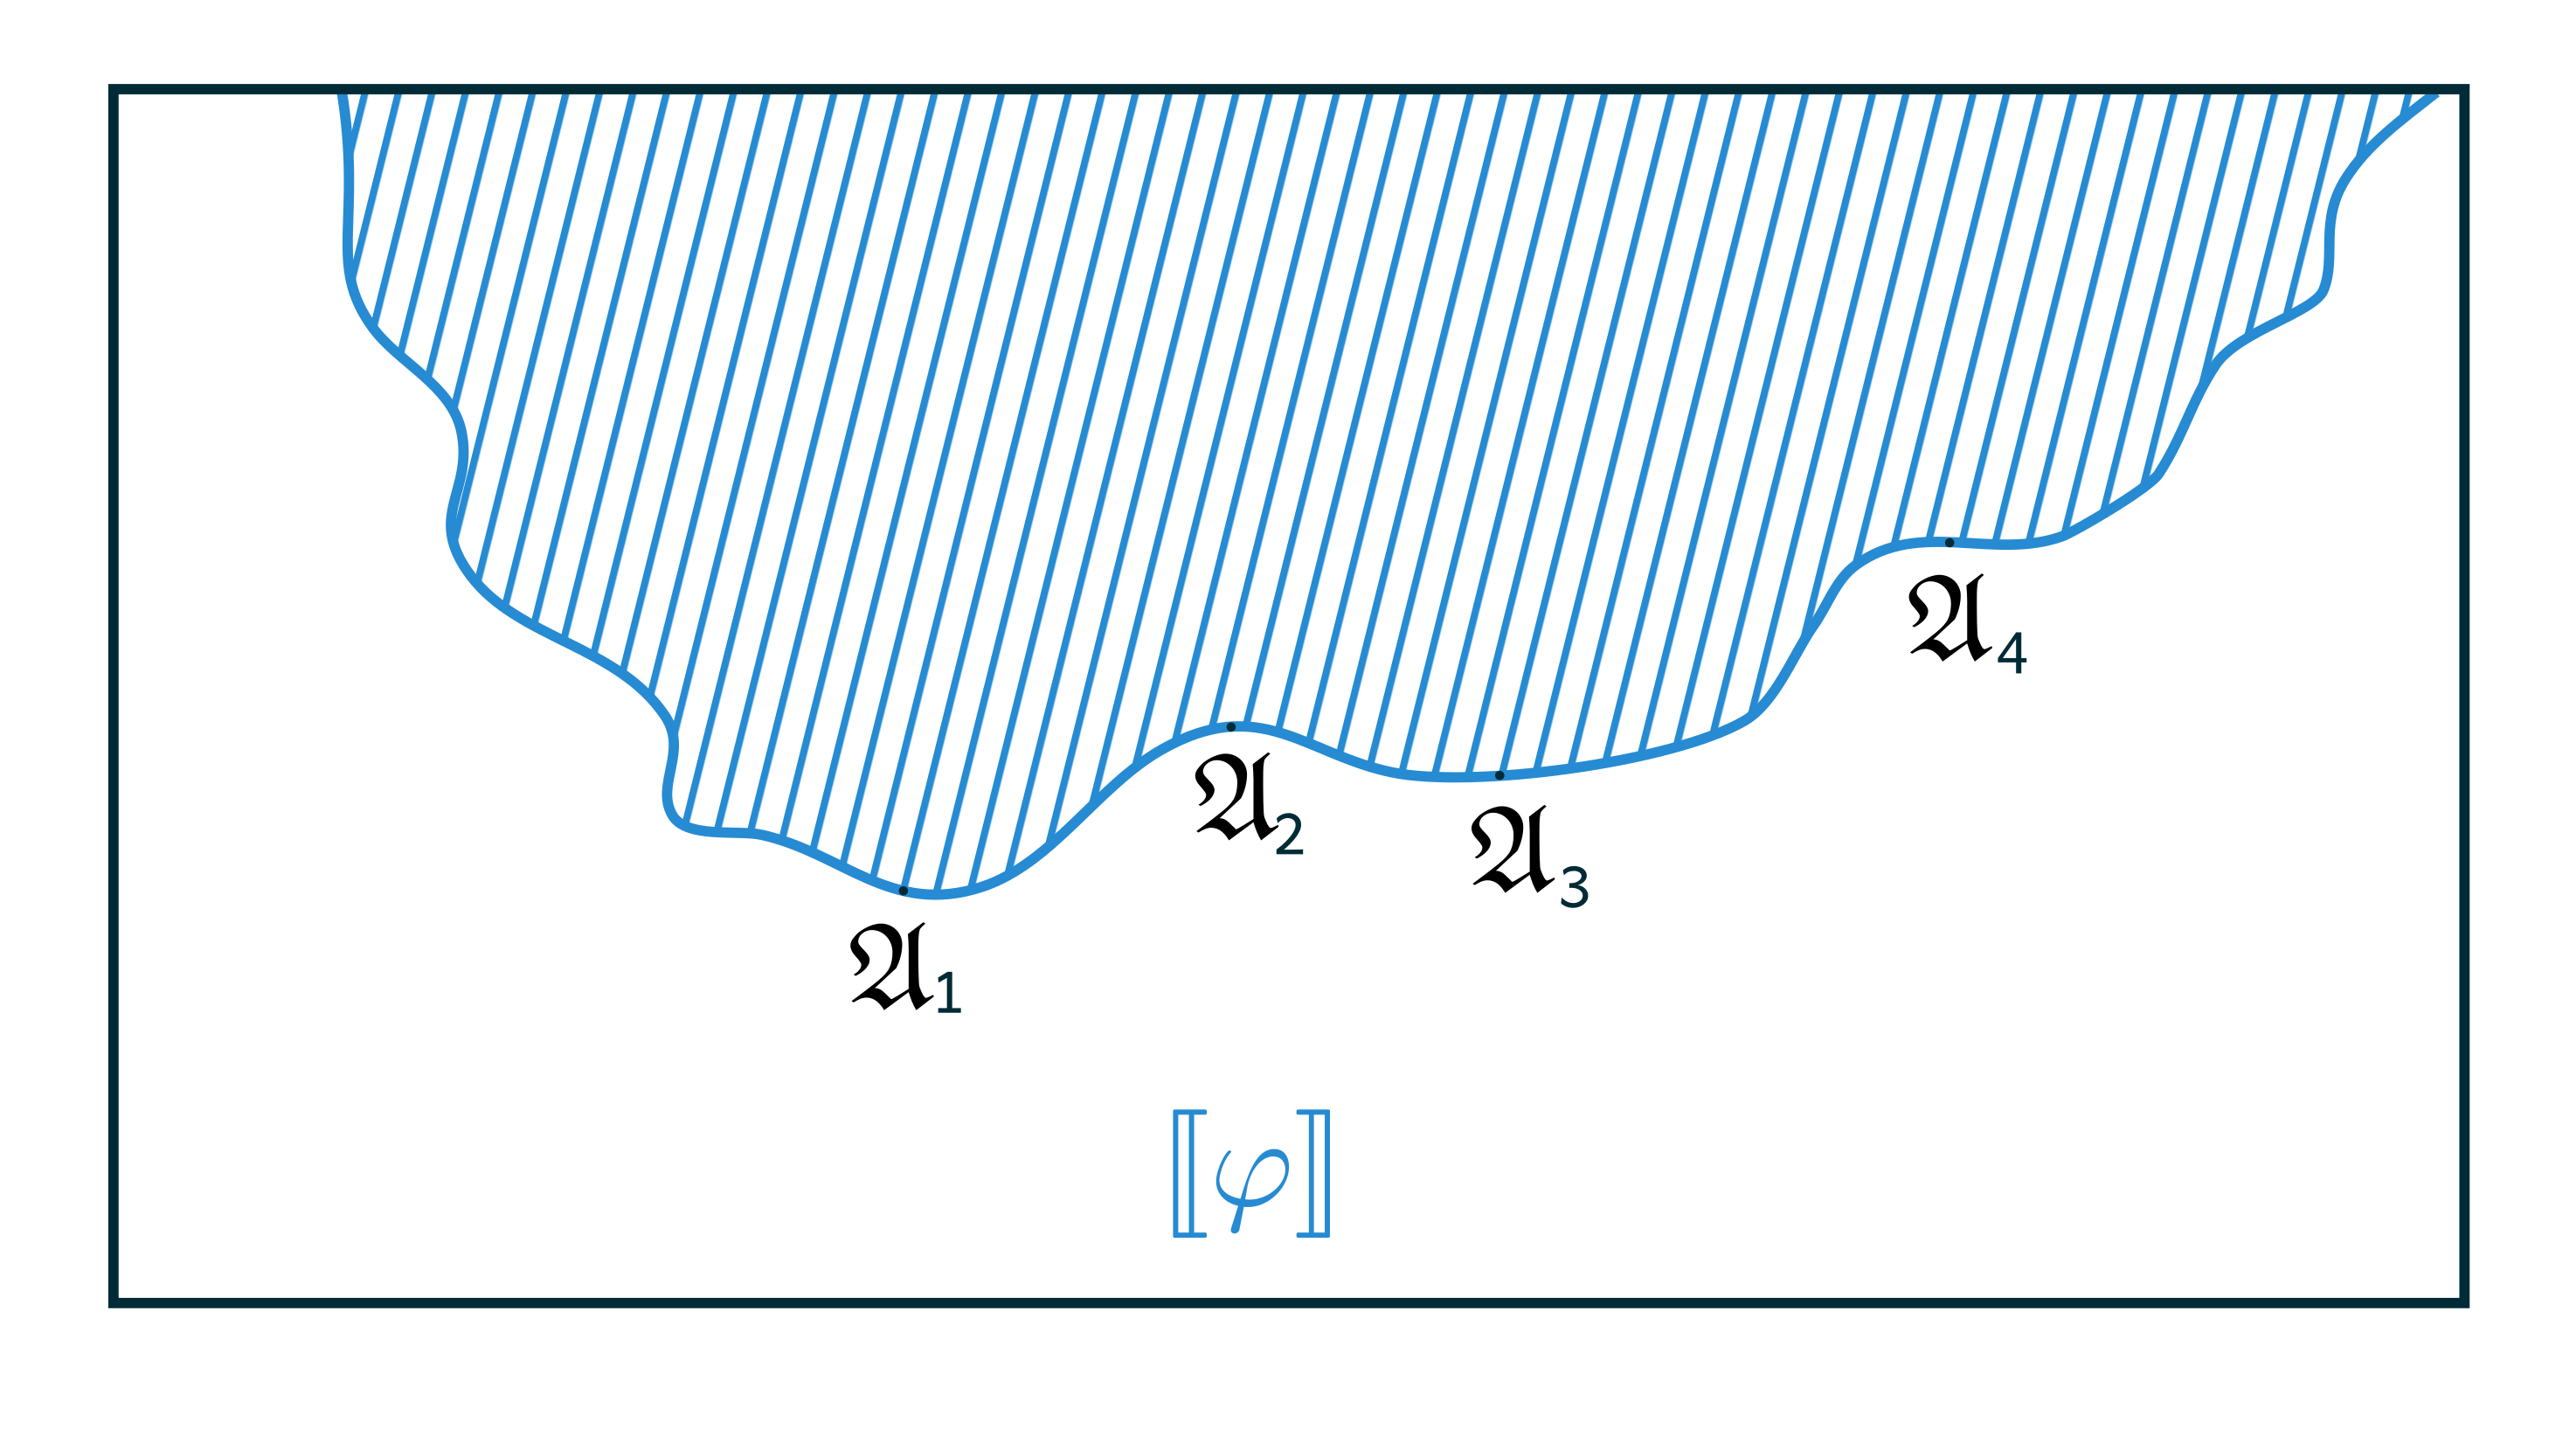
\includegraphics[width=8cm]{figures/quizz_Page 12.png}
    \end{center}
    \pause
    \begin{itemize}
        \item List minimal models of $\varphi$
        \item Assume that $\model{A} \models \varphi$ is extremely large
        \item Construct $\model{B} \isubleq \model{A}$ that continues
            to satisfy $\varphi$, but is smaller.
        \item Conclude.
    \end{itemize}
\end{frame}


\begin{frame}{The best ``generic'' result prior to this work}
    \begin{theorem}[\cite{ADG08}]
        \vspace{0.1em}
        Let $\mathcal{C}$ be a \textbf{hereditary} class of finite structures
        closed under \textbf{disjoint unions}.
        Then, item $1$ implies item $2$:
        \begin{enumerate}
            \item $\mathcal{C}$ has \emph{bounded degree},
            \item The Łoś-Tarski theorem relativises to $\mathcal{C}$.
        \end{enumerate}
    \end{theorem}
    \pause
    \begin{block}{Works for infinitely many classes}
    \end{block}
\end{frame}

\section{The results}\label{the-results}

\subsection{Localisations}\label{localisations}

\begin{frame}{Main theorem}

    \begin{theorem}[The localisation theorem]
        \vspace{0.1em}
        Let $\mathcal{C}$ be a \textbf{hereditary} class of finite structures
        closed under \textbf{disjoint unions}.
        Then, the following are equivalent:
        \begin{enumerate}
            \item The Łoś-Tarski theorem relativises to $\mathcal{C}$,
            \item The Łoś-Tarski theorem \textbf{locally} relativises to $\mathcal{C}$.
        \end{enumerate}
    \end{theorem}

    \pause

    \begin{block}{Remarks}
        \begin{itemize}
            \item Is now an equivalence.
            \item Strictly generalises \cite{ADG08}.
        \end{itemize}
    \end{block}
\end{frame}

\subsection{Locality???}

\begin{frame}{What is a neighbourhood?}
    \begin{center}
        \centering
        \foreach[count=\xi] \i in {13,14,15} {%
            \only<\xi>{%
                \includegraphics[width=12cm]{figures/quizz_Page \i.png}%
            }%
        }
    \end{center}
\end{frame}

\begin{frame}{What is a localisation?}
    \begin{equation*}
        \Loc{\mathcal{C}}{k}{r} \defined
        \setof{
            \Neighb{\model{A}}{\vec{a}}{r}
        }{
            \vec{a} \in \model{A}^k
        }
        \quad .
    \end{equation*}
    \pause
    \begin{alertblock}{Remark for finite classes}
        \begin{equation*}
            \mathcal{C} = \bigcup_{k,r} \Loc{\mathcal{C}}{k}{r} \quad .
        \end{equation*}
    \end{alertblock}
\end{frame}

\begin{frame}{Example of localisations}
    \begin{equation*}
        \Loc{\Cycles}{1}{3} = ? 
    \end{equation*}
    \pause
    \begin{center}
        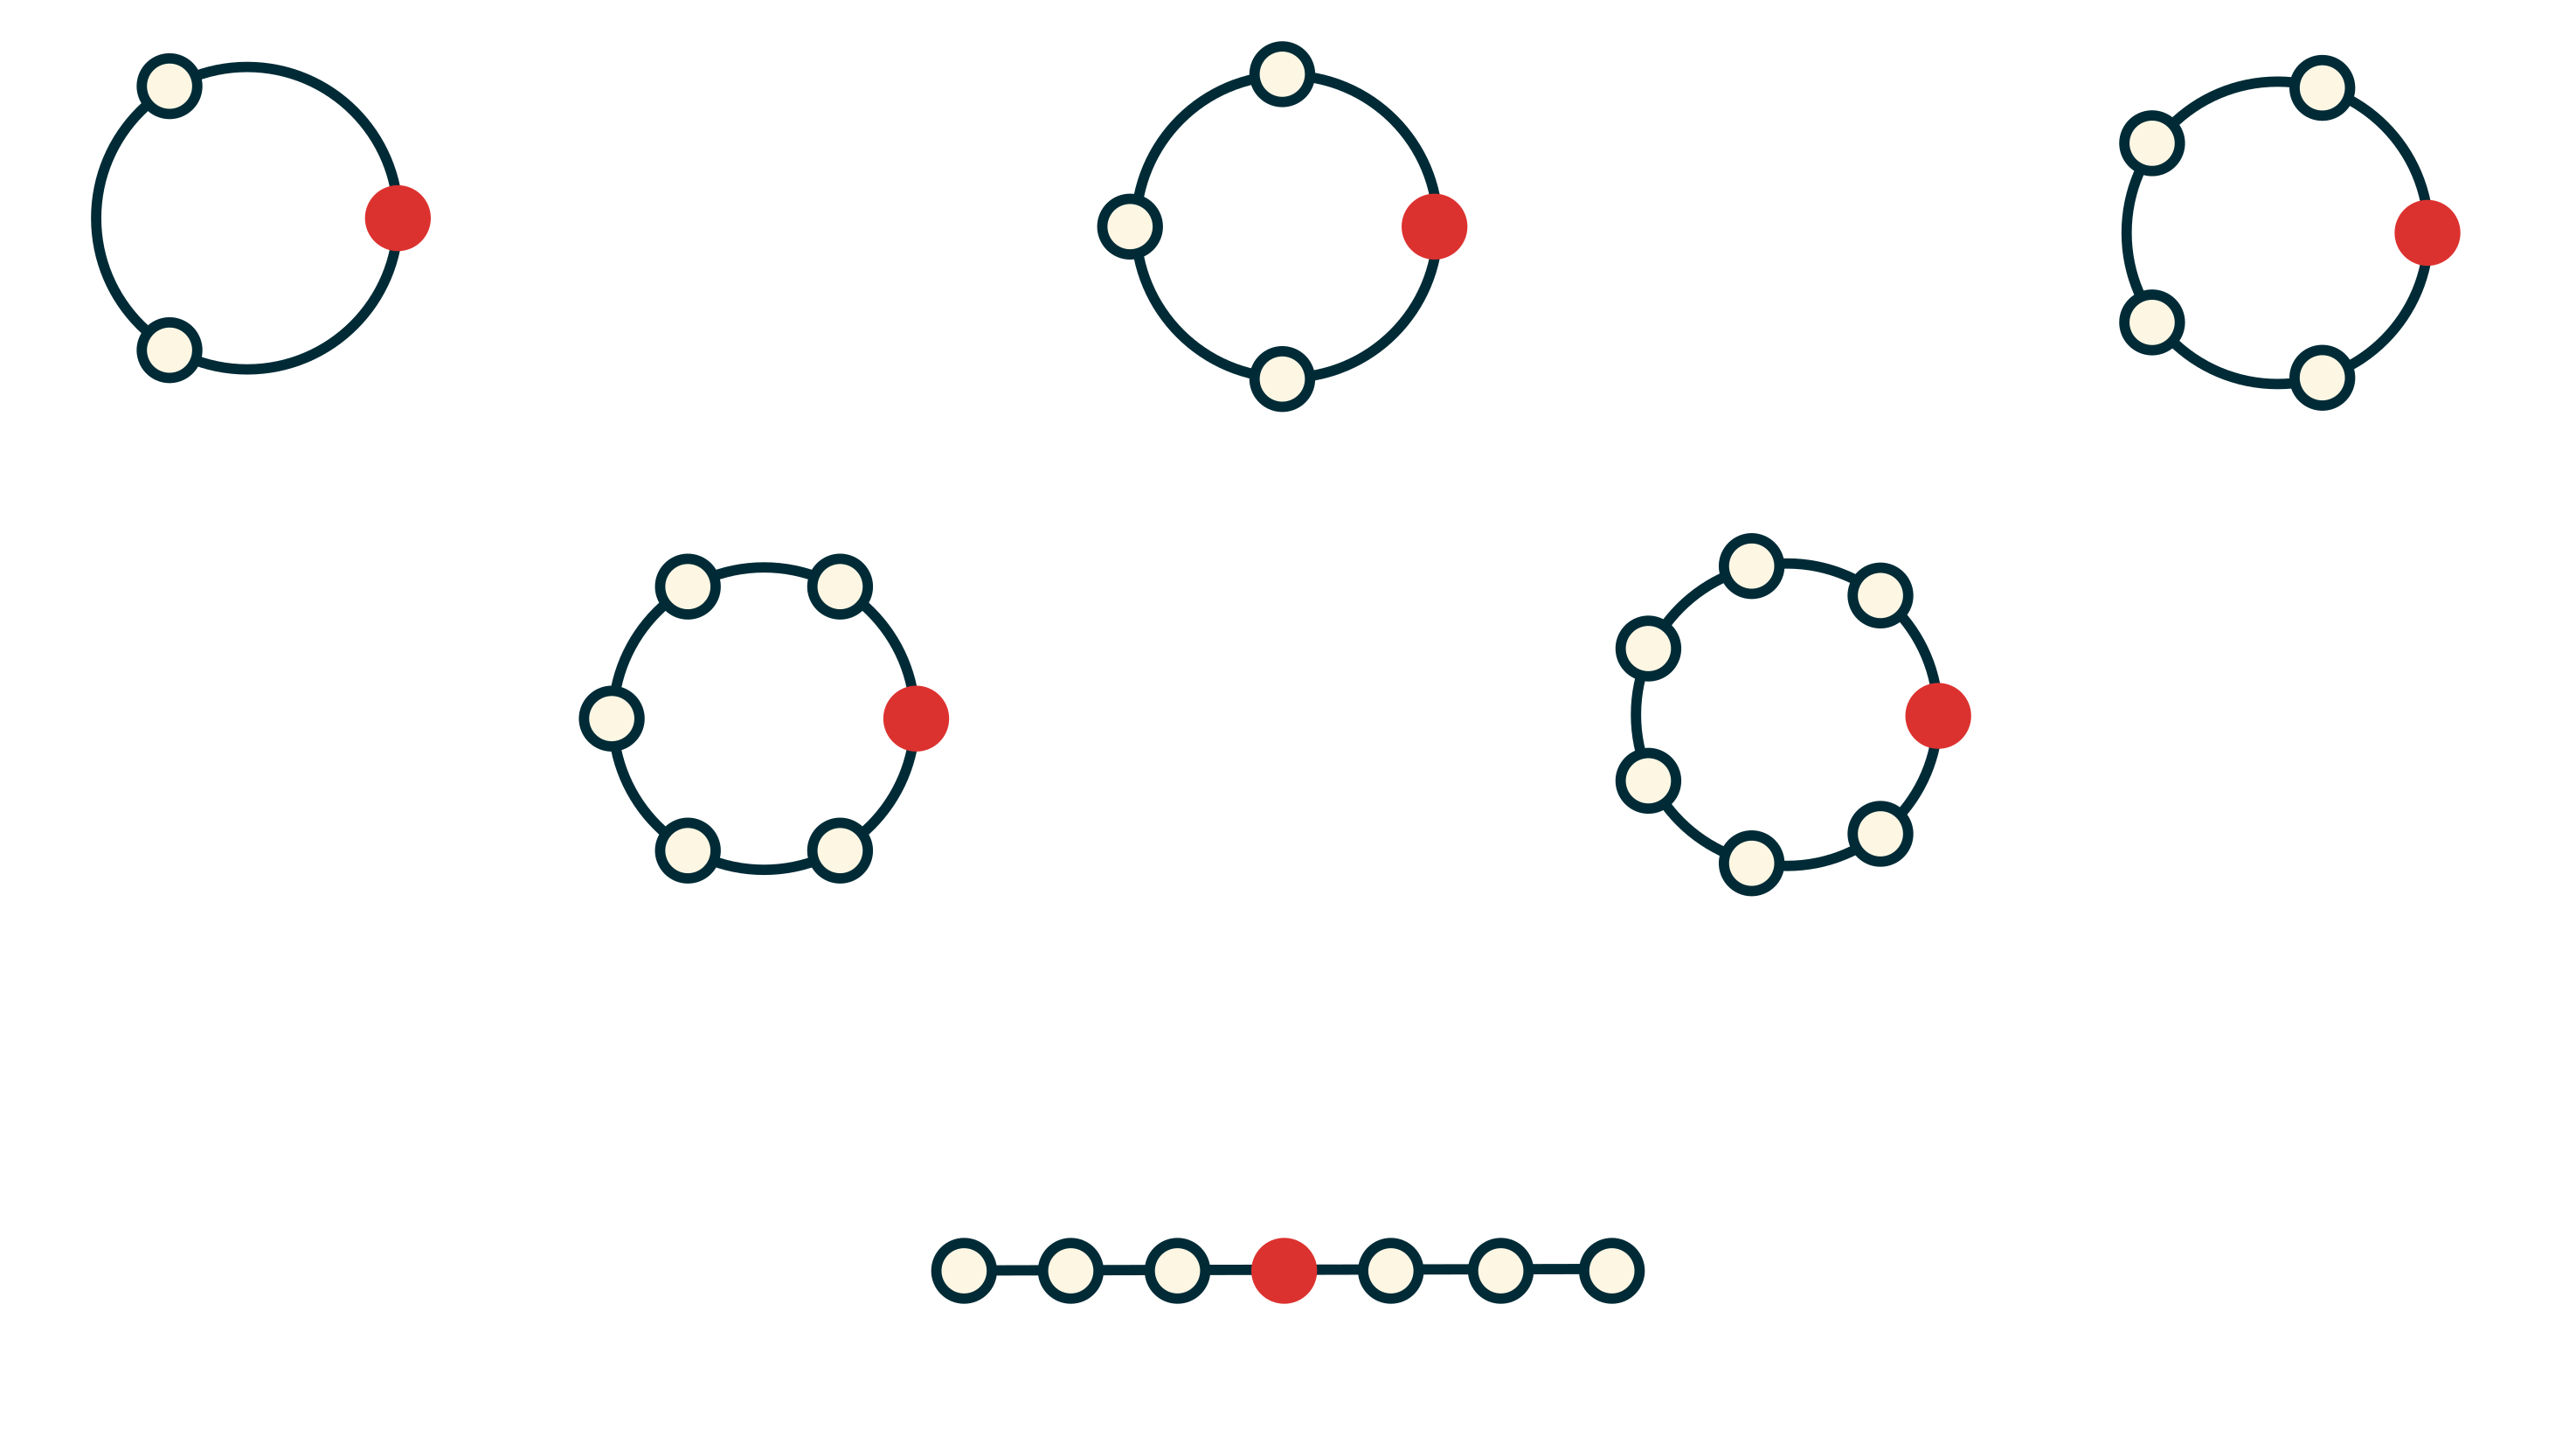
\includegraphics[width=8cm]{figures/quizz_Page 16.png}
    \end{center}
\end{frame}

\begin{frame}{Example of localisations}
    \begin{alertblock}{Locally finite?}
        \centering
        $\mathcal{C}$ has bounded degree
        $\iff$
        $\Loc{\mathcal{C}}{k}{r}$ is finite for all $r,k \geq 0$.
    \end{alertblock}
\end{frame}

\begin{frame}{How do we use such a theorem?}
    \begin{center}
        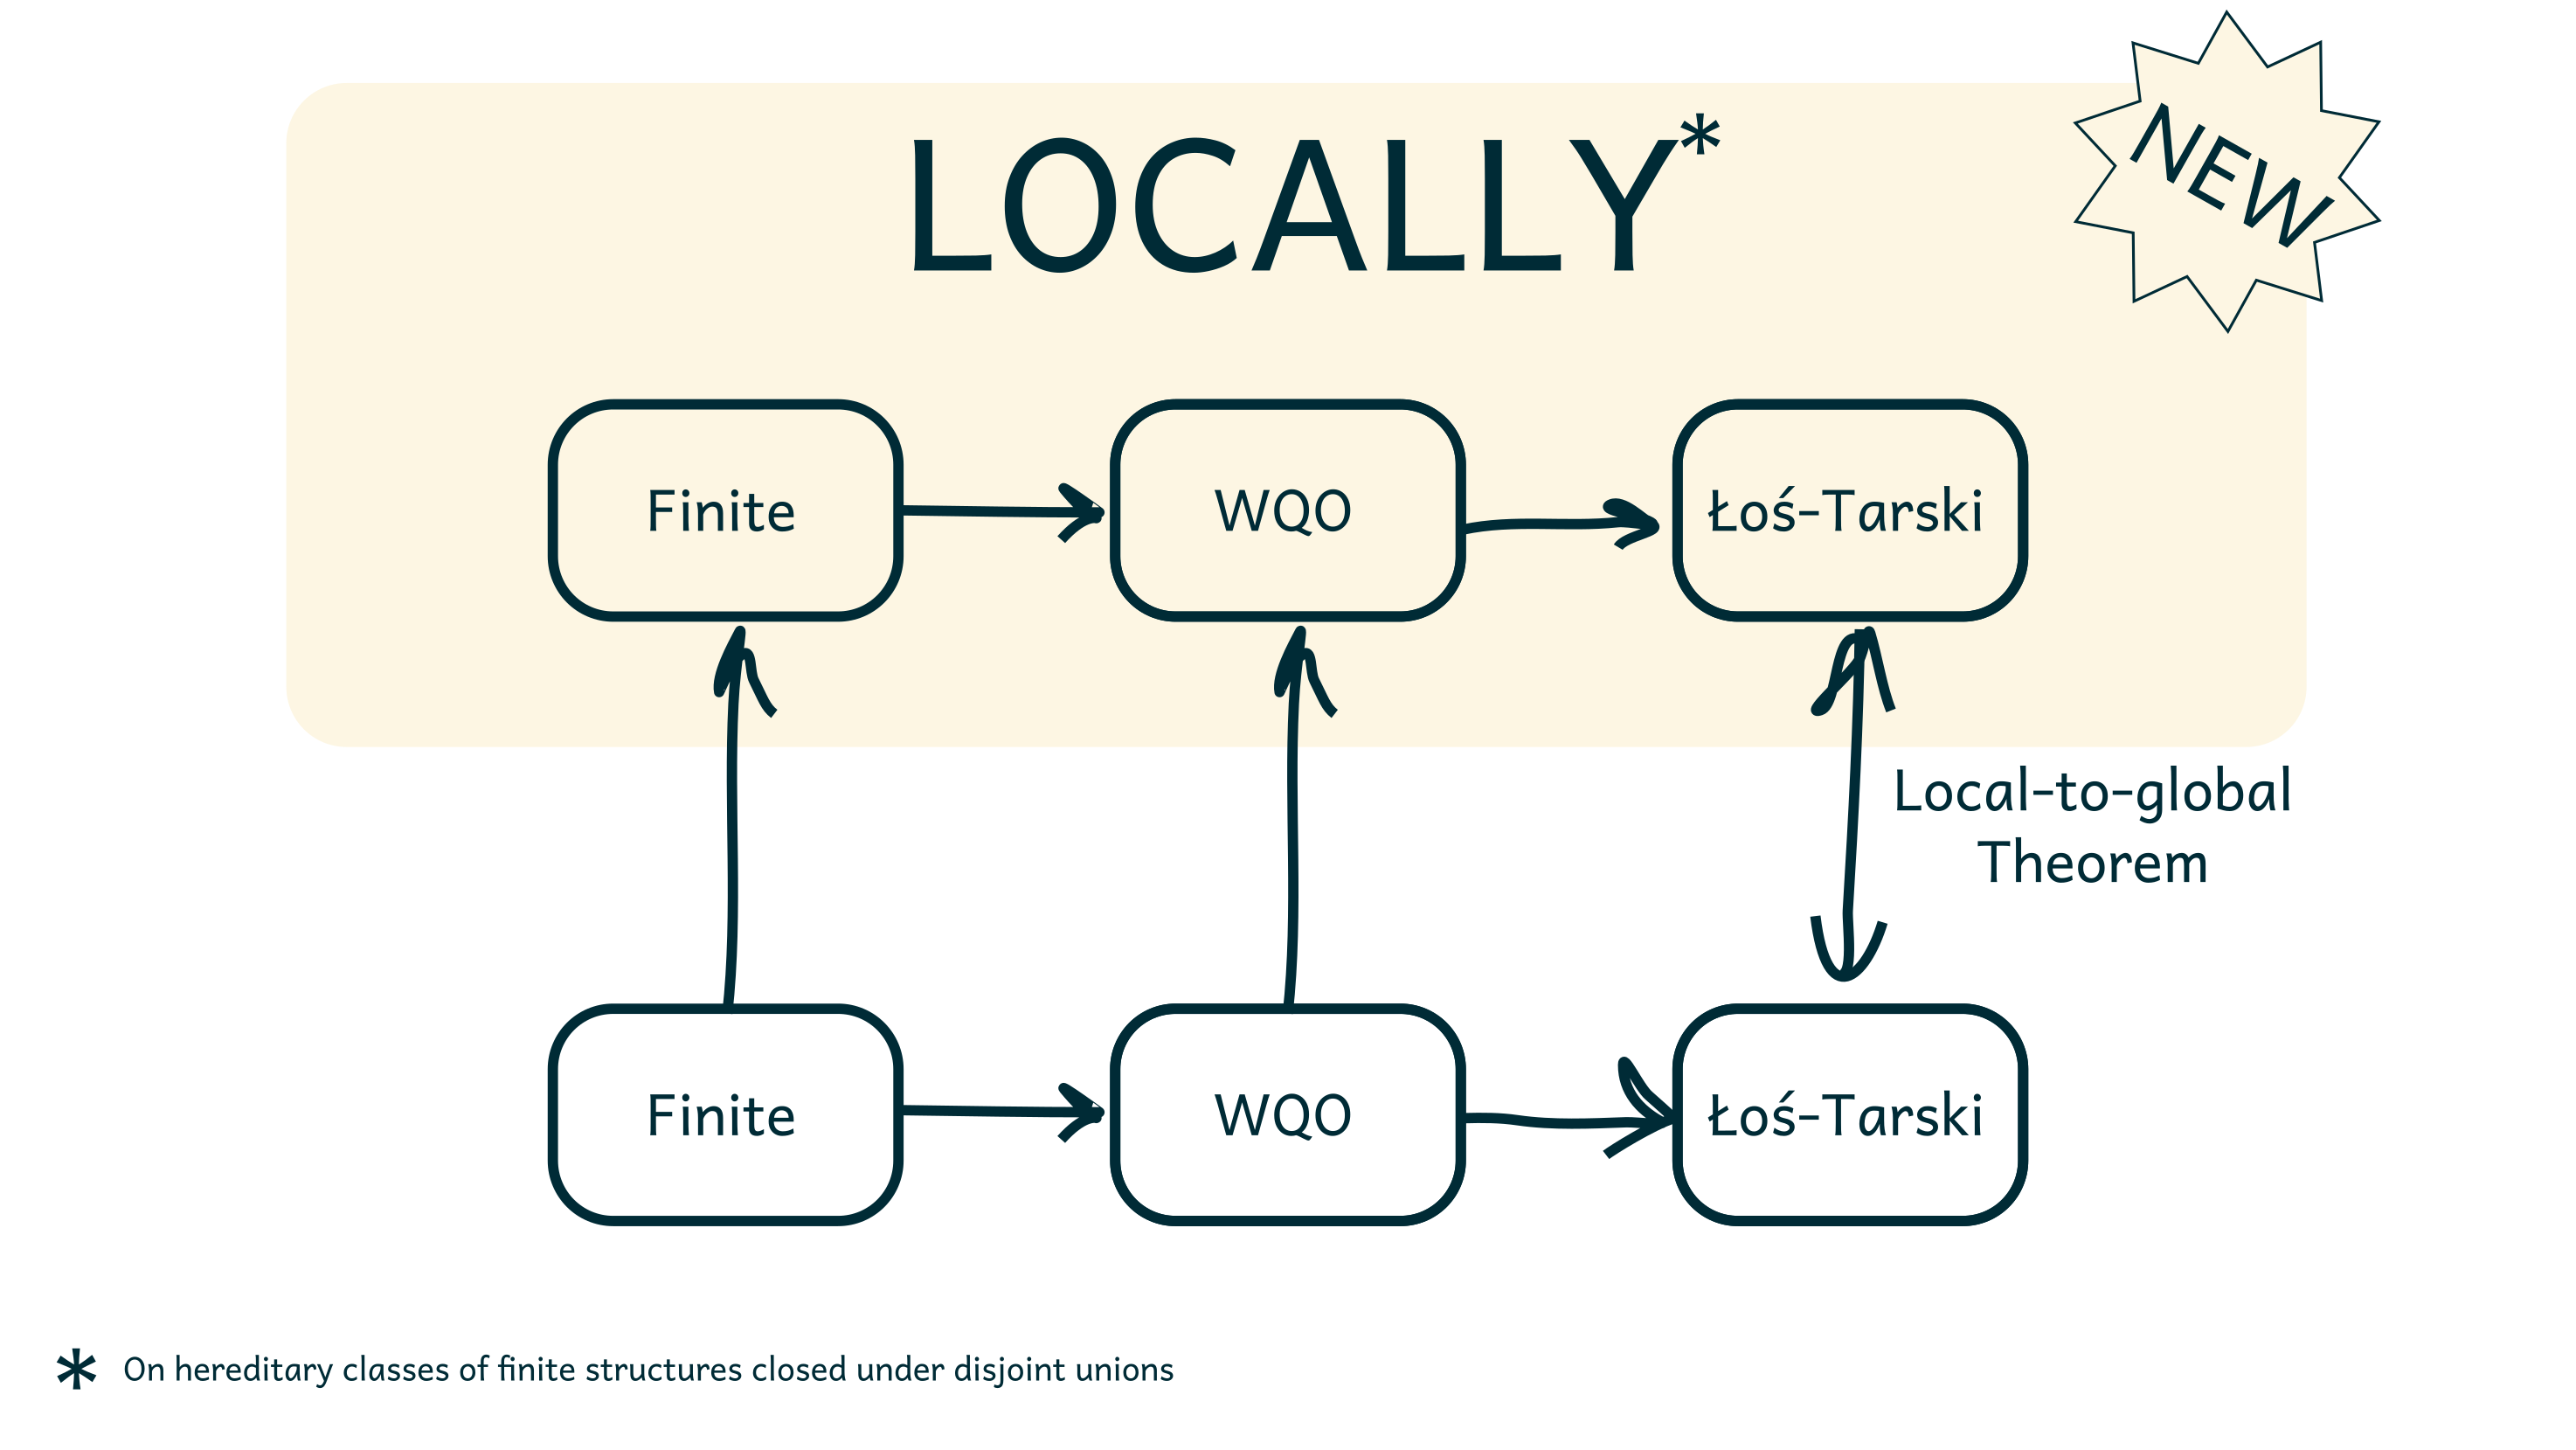
\includegraphics[width=15cm]{figures/quizz_Page 17.png}
    \end{center}
\end{frame}

\section{The proofs}\label{the-proofs}

\subsection{Positive Locality and Neighbourhroods}

\begin{frame}[standout]
    Until now, we never really used $\FO$!
\end{frame}

\subsubsection{Local formulas}\label{local-formulas}

\begin{frame}{Local formulas}
    \begin{block}{$r$-local formulas $\varphi(x)$}
        \begin{equation*}
            \model{A} \models \varphi(a)
            \iff
            \Neighb{\model{A}}{a}{r} \models \varphi(a)
            \quad
        \end{equation*}
    \end{block}
    \pause
    \begin{alertblock}{What about sentences?}
        \vspace{0.1em}
        \begin{itemize}
            \item \textbf{Basic local sentences} \cite{GAIF82}
                ($\varphi(x)$ is $r$-local)
        \begin{equation*}
            \exists^{\geq n}_{r} x. \varphi(x) \quad .
        \end{equation*}
    \item \textbf{Existential-local sentences} ($\varphi(\vec{x})$ is $r$-local)
        \begin{equation*}
            \exists \vec{x}. \varphi(\vec{x}) \quad .
        \end{equation*}
        \end{itemize}
    \end{alertblock}
\end{frame}

\begin{frame}{Evaluating a basic local sentence}
    \begin{equation*}
            \exists^{\geq n}_{r} x. \varphi(x) \quad .
    \end{equation*}
    \begin{enumerate}
        \item For each node $a \in \model{A}$, decide whether
            $\Neighb{\model{A}}{a}{r} \models \varphi(a)$.
        \item Decide if there exists a set of at least $n$ points
            with non-intersecting $r$ neighbourhoods that 
            locally satisfy $\varphi$
            ($r$-independent set).
    \end{enumerate}
\end{frame}

\begin{frame}{Positive Locality}
    \begin{theorem}[\cite{GAIF82}]
        \vspace{0.1em}
        Every sentence \(\varphi\) is
        equivalent to a Boolean combination of basic local sentences.
    \end{theorem}

    \pause
    \vspace{1em}
    \hrule
    \vspace{0.8em}

    \begin{theorem}[Positive Locality]
        \vspace{0.1em}
        For every sentence \(\varphi\), the following are
        equivalent:

        \begin{enumerate}
        \tightlist
        \item
          \(\varphi\) is equivalent to a \textbf{positive} Boolean combination
          of basic local sentences.
        \item
          \(\varphi\) is equivalent to an existential local sentence.
        \end{enumerate}
    \end{theorem}
\end{frame}

\subsection{Combinatorics of
Neighbourhroods}\label{combinatorics-of-neighbourhroods}

\begin{frame}{Existential Local Łoś-Tarski}
    \begin{theorem}
        \vspace{0.1em}
        Let $\mathcal{C}$ be a \textbf{hereditary} class of finite structures
        closed under \textbf{disjoint unions}.
        Then, the following are equivalent:
        \begin{enumerate}
            \item 
                Łoś-Tarski \textbf{locally} relativises to
                $\mathcal{C}$,
            \item 
                Existential local sentences that are
                preserved under extensions over $\mathcal{C}$
                are equivalent to existential sentences.
        \end{enumerate}
    \end{theorem}
    \pause
    \begin{equation*}
        (k,r)-\text{Existential local over } \mathcal{C}
        \leftrightarrow
        \text{ Sentence over } \Loc{\mathcal{C}}{k}{r}
        \quad .
    \end{equation*}
\end{frame}

\begin{frame}{The main idea}
    \begin{alertblock}{To conclude it suffices to prove that ...}
        \vspace{0.1em}
        Sentences preserved under extensions
        are equivalent to existential local sentences.
    \end{alertblock}
    \pause
    \begin{block}{Replacing ``finite size" with ``bounded radius"}
        \vspace{0.1em}
        \begin{itemize}
            \item Consider a minimal model $\model{A}$ of a sentence $\varphi$
                and assume that it is very \emph{sparse}
            \item Extract a substructure $\model{B} \isubleq \model{A}$
                that satisfies $\varphi$.
            \item Conclude.
        \end{itemize}
    \end{block}
\end{frame}

\subsection{The core combinatorial argument}


\begin{frame}{First attempt}
    \begin{enumerate}
        \item 
            Consider a first order sentence \(\varphi := \bigvee_i \bigwedge_k
            \theta_{i,k}^+ \wedge \bigwedge_k \neg \theta_{i,k}^-\) preserved
            under extensions in Gaifman normal form, with locality radius $r$.

        \item
            Take $\model{A}$ a minimal model of $\varphi$.

        \item 
            Consider the \emph{positive} witnesses $\vec{a}$ of $\model{A}$.

        \item 
            Construct $\model{B} \defined \Neighb{\model{A}}{\vec{a}}{r}$.

        \item \textbf{Hope:} $\model{B} \models \varphi$.
    \end{enumerate}
\end{frame}

\begin{frame}{Problem}
    \begin{center}
        The neighbourhoods in 
        $\Neighb{\model{A}}{\vec{a}}{r}$
        are obtained as \emph{intersections}
        of neighbourhoods of $\model{A}$.
    \end{center}

    \begin{center}
        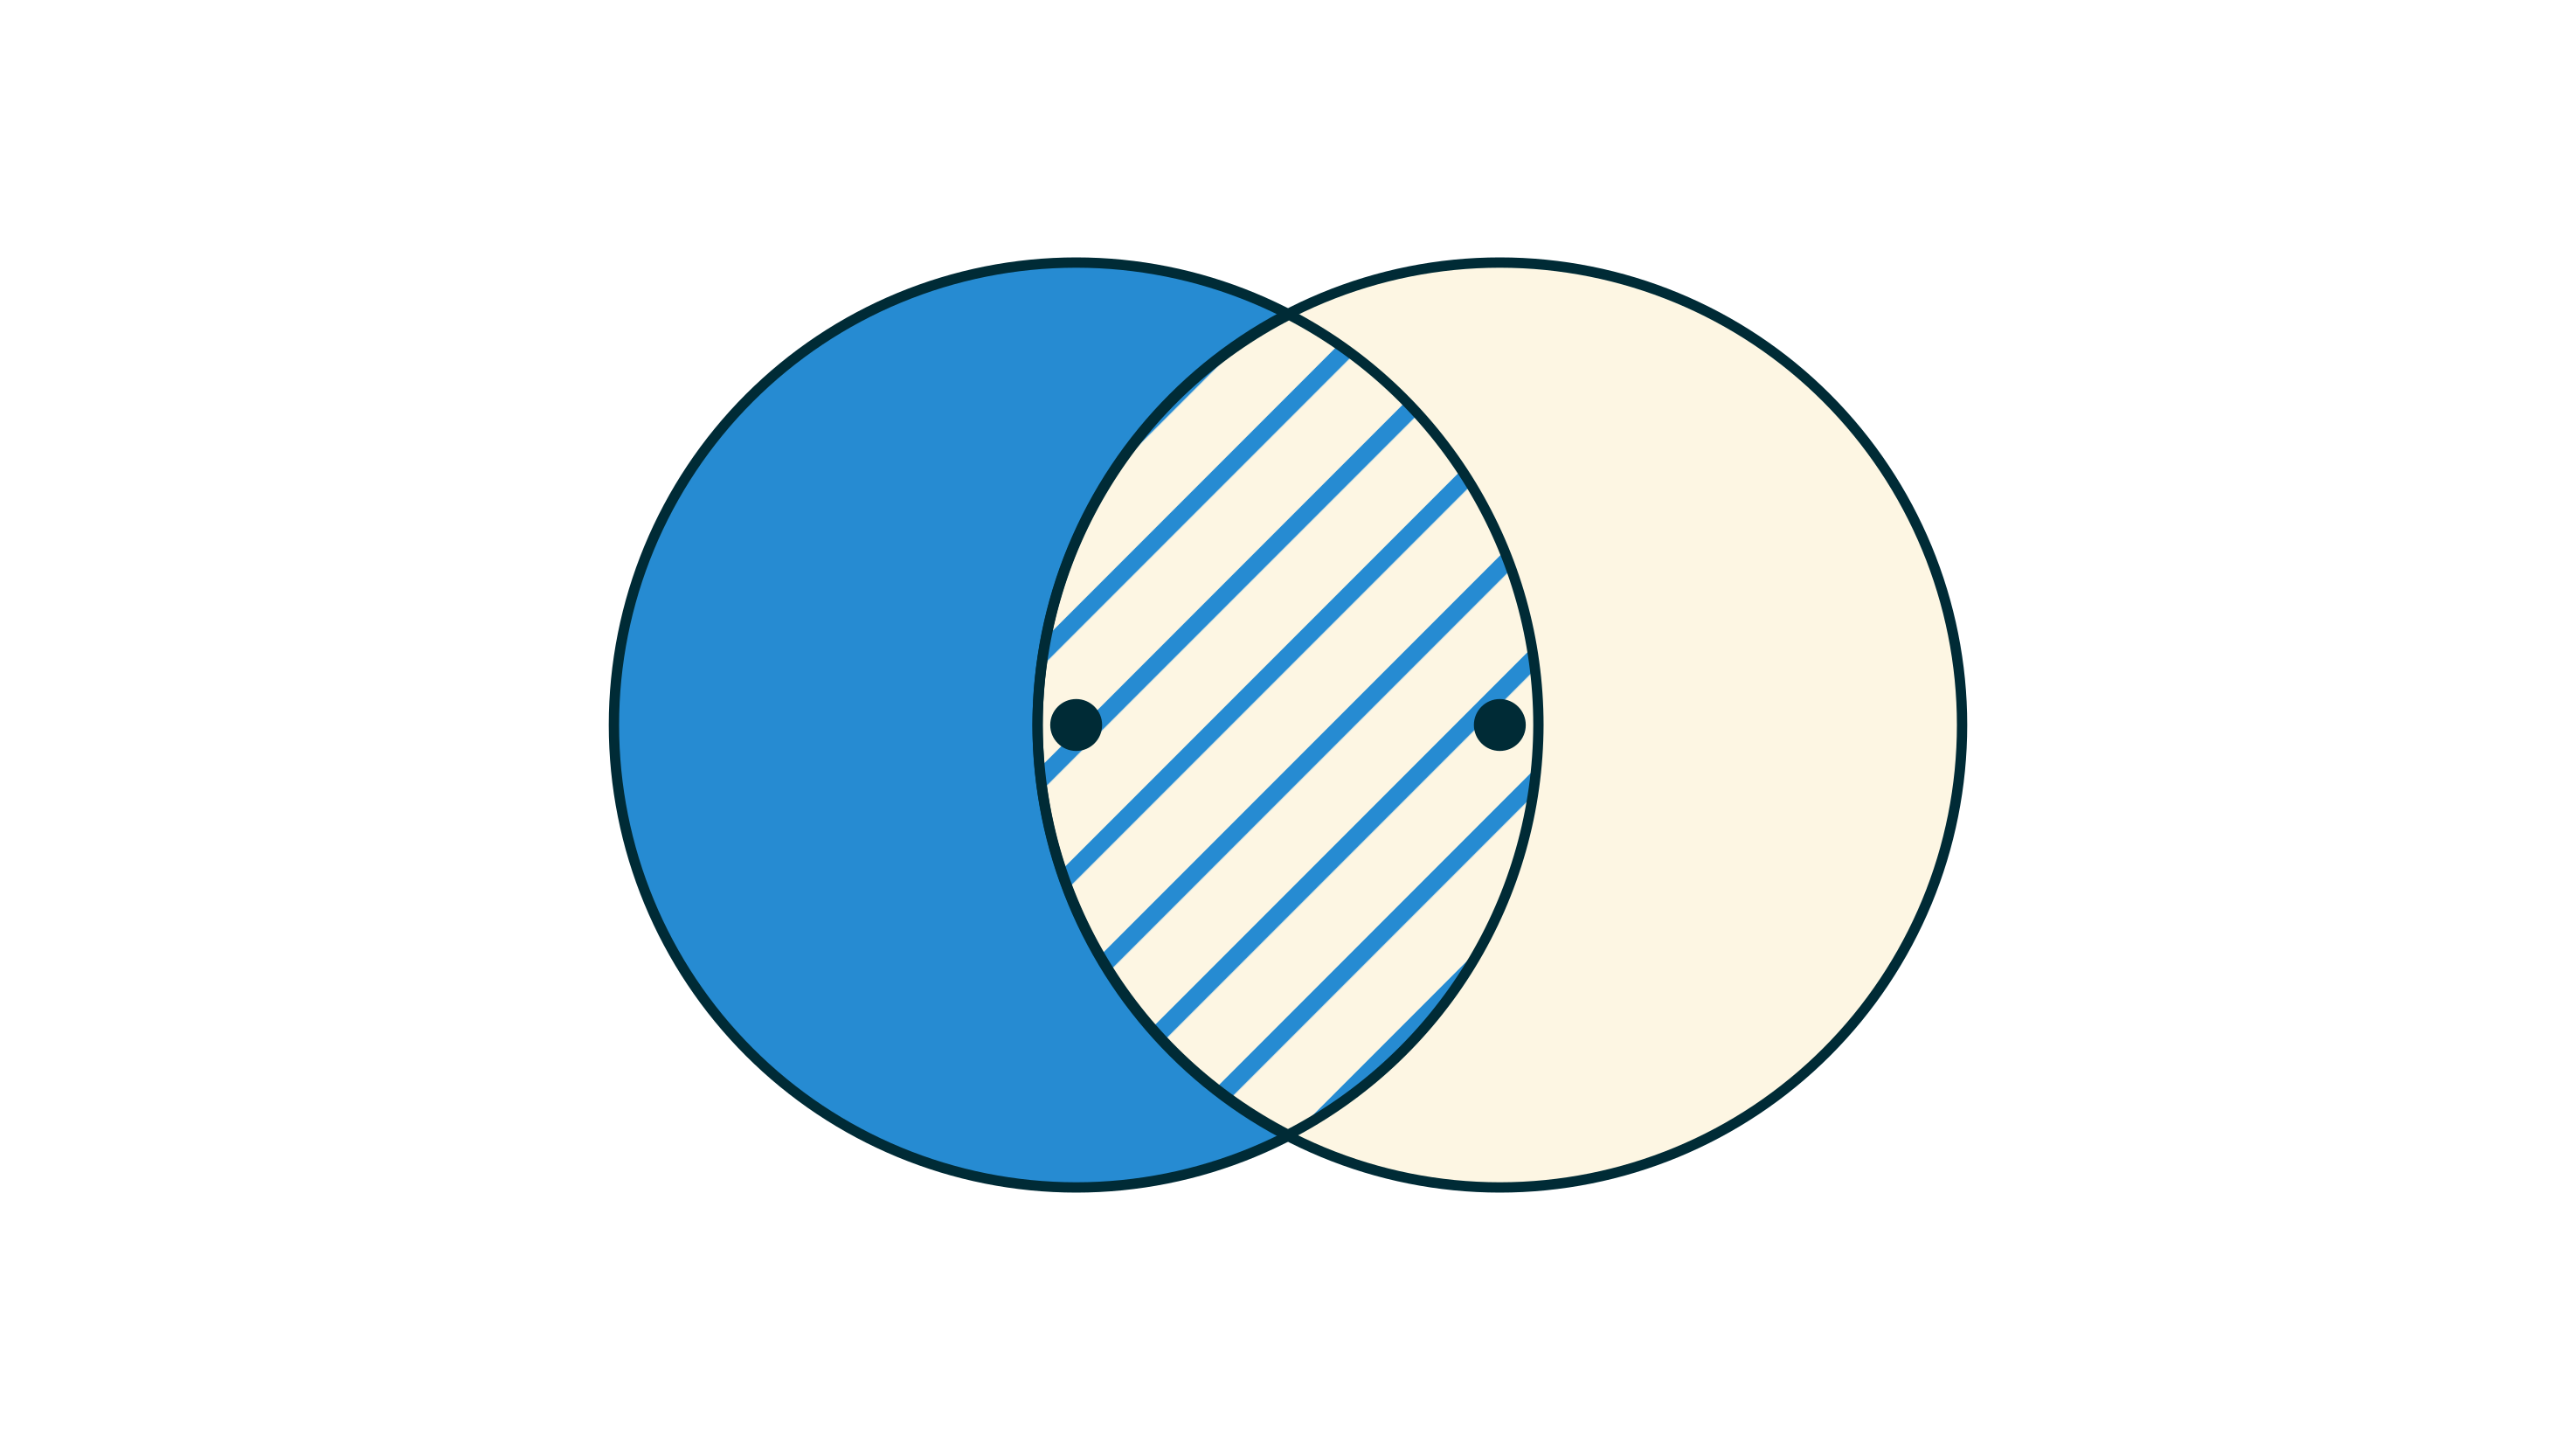
\includegraphics[width=10cm]{figures/quizz_Page 18.png}
    \end{center}
\end{frame}

\begin{frame}{Solution}
    \begin{alertblock}{Use monadic second order logic}
        \vspace{0.1em}
        Encode the intersections using monadic second order formulas:
        \(\exists X. \psi_{|X}\).
    \end{alertblock}

    \begin{alertblock}{Cluster the witnesses in one large neighbourhood}
    \end{alertblock}
\end{frame}

\begin{frame}{A graph theoretic result}
    \begin{lemma}[Frequent and rare colours]
        \vspace{0.1em}
        Let $N,r,k \in \Nat$. There exists bounds
        $K_m \geq k$ and $R_m \geq r$
        such that for all graphs $H$ with $N$ colours,
        there exist $r \leq R \leq R_m$,
        $k \leq K \leq K_m$, subsets $C^H$ and $G^H$
        of $H$ such that the following holds:
        \begin{enumerate}[<+->]
            \item Both $C^H$ and $G^H$ have size at most $K_m$;
            \item The sets $C^H$ and $G^H$ have non-intersecting $R$-neighbourhoods;
            \item Elements in $C^H$ have non-intersecting $R$-neighbourhoods;
            \item For every colour $c \in \set{1, \dots, N}$,
                one of the following holds:
                \begin{enumerate}
                    \item All nodes $x \in H$  with colour $c$
                        satisfy $\Neighb{H}{x}{r} \subseteq \Neighb{H}{C^H}{R}$;
                    \item There are at least $k$ distinct element in $G^H$
                        with colour $c$.
                \end{enumerate}
        \end{enumerate}
    \end{lemma}
\end{frame}

\begin{frame}
    \centering
    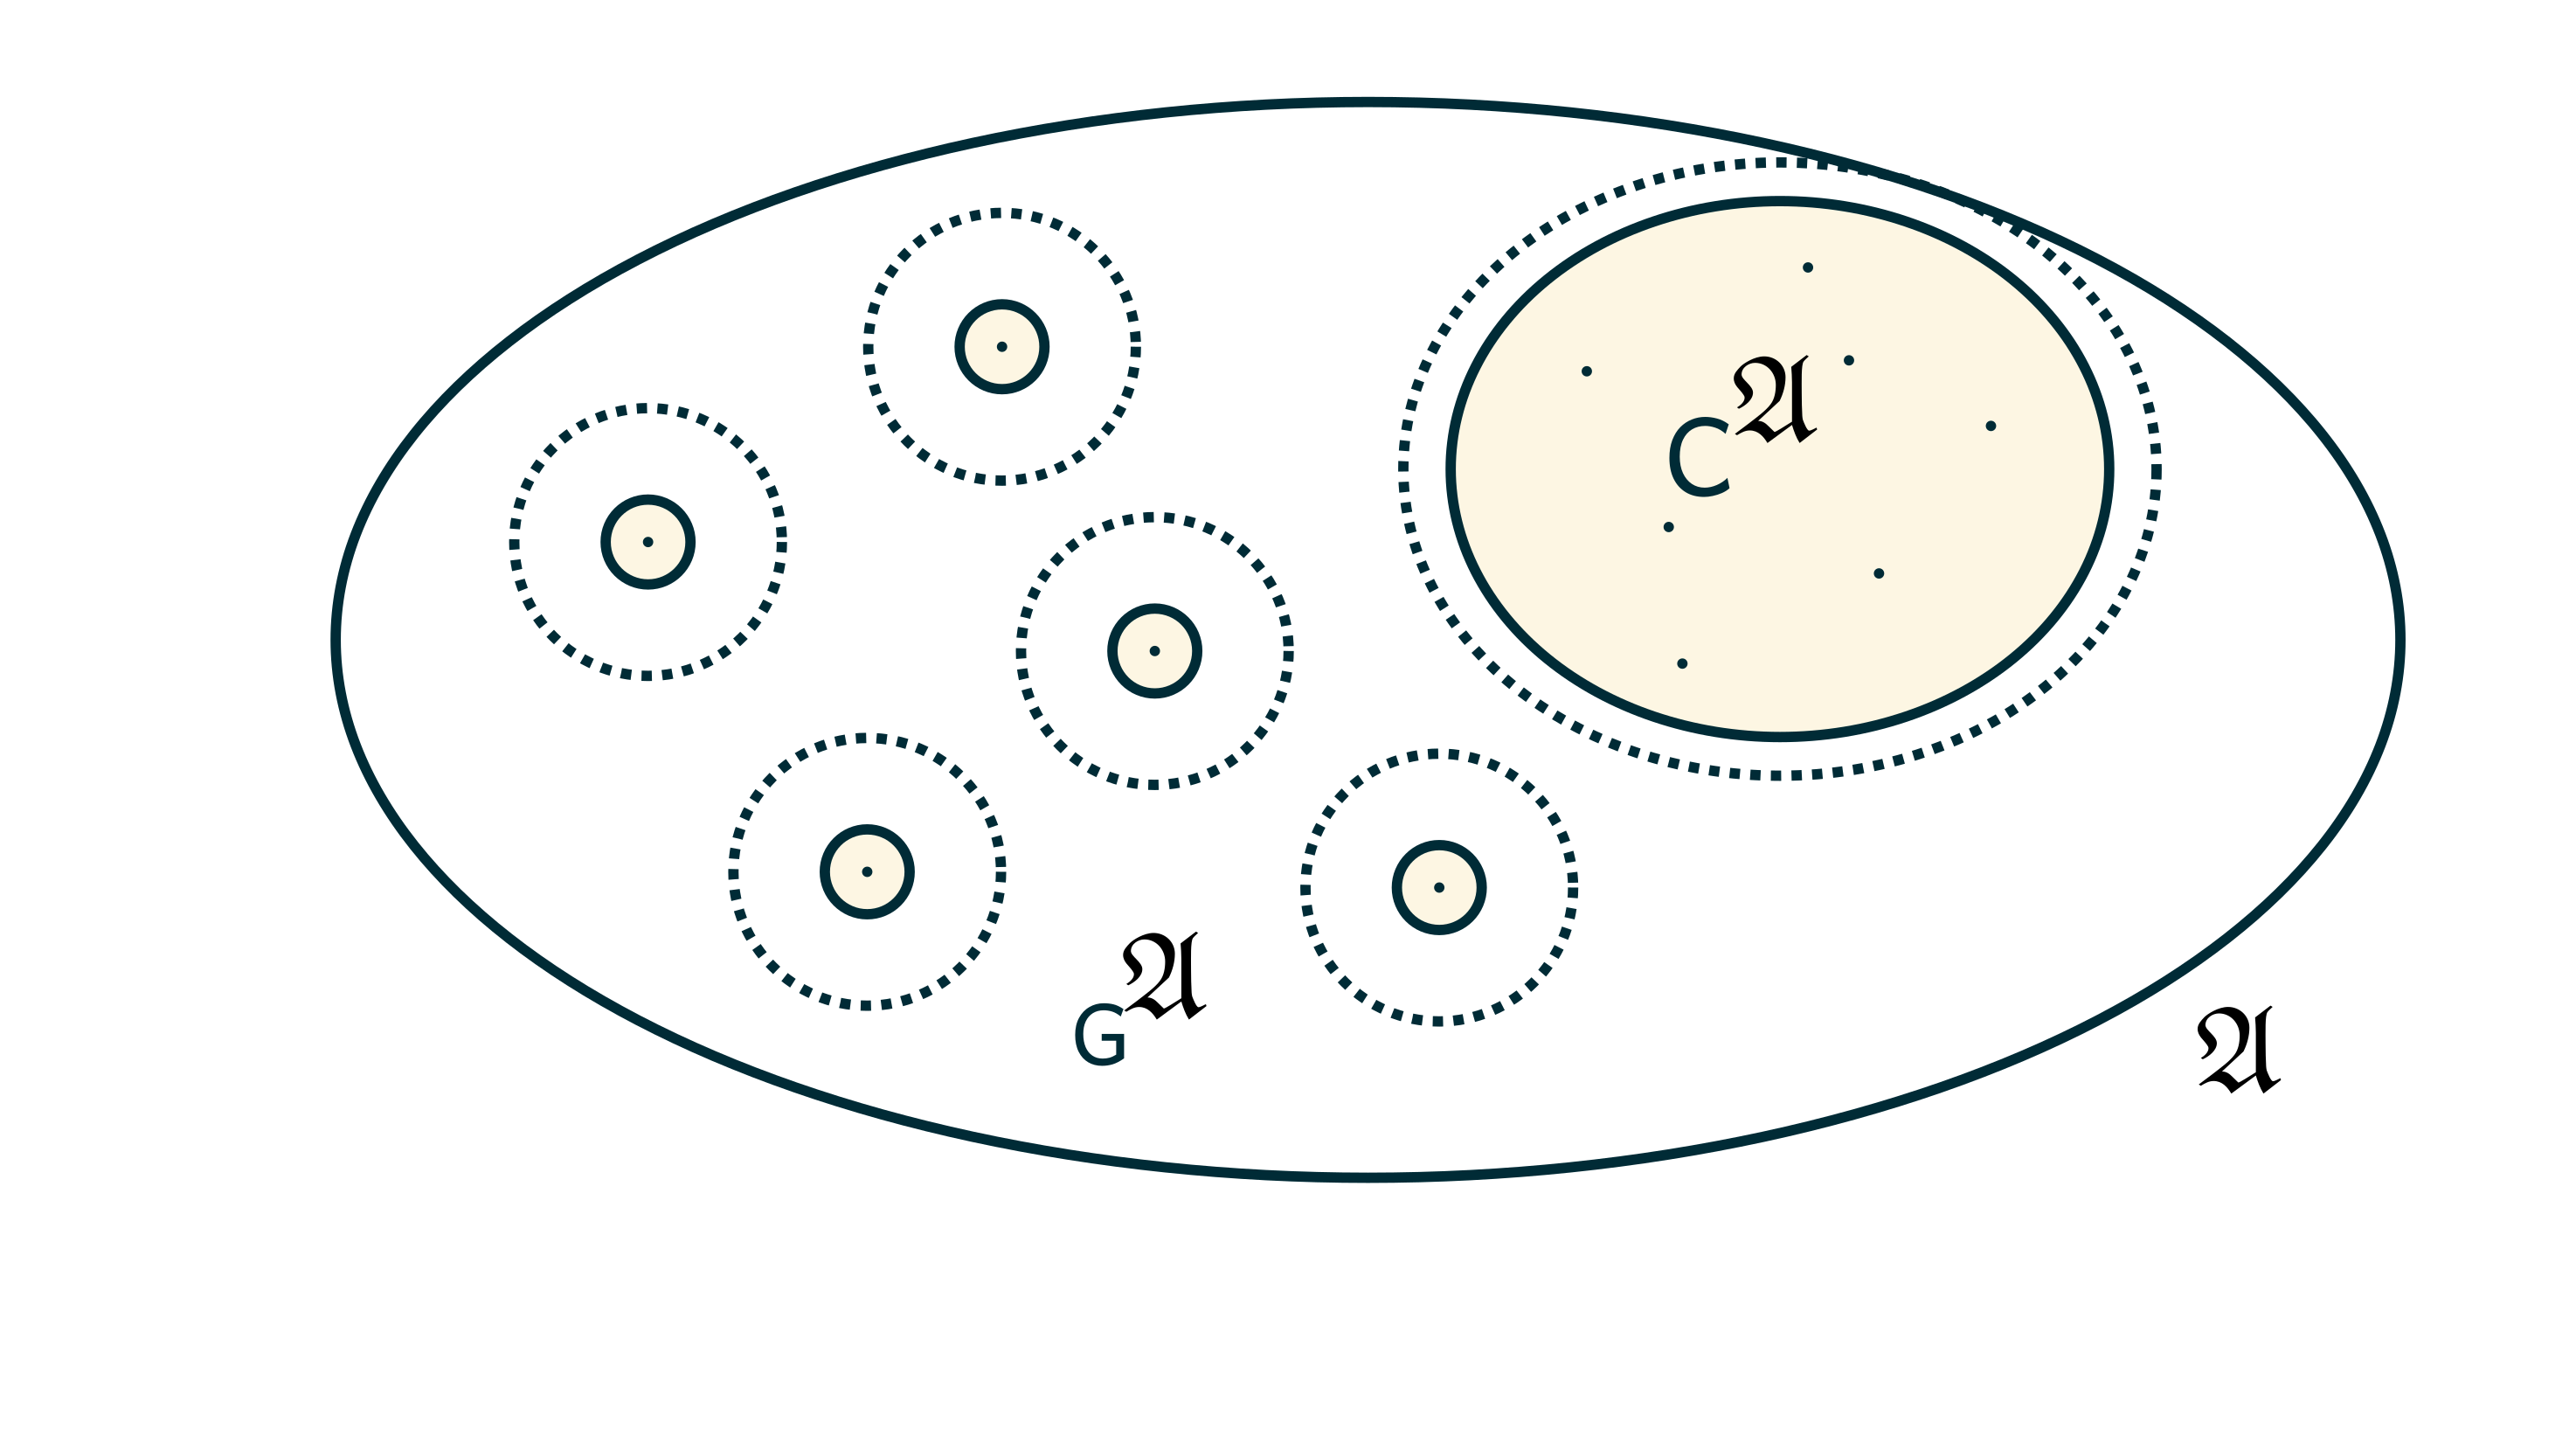
\includegraphics[width=10cm]{figures/quizz_Page 19.png}
\end{frame}

\begin{frame}{Actual Proof \hfill (simplified)}
    \begin{itemize}[<+->]
        \item Consider a sentence $\varphi$ in Gaifman normal form,
            with quantifier rank $q$, of locality radius $r$,
            and searching for independent sets of size $k$.
        \item Consider a minimal model $\model{A}$ of $\varphi$.
        \item Colour the nodes of $\model{A}$ with
            the collection of all $\MSO(q,k)$
            formulas satisfied on their $r$-local neighbourhood.
        \item Apply the combinatorial lemma.
        \item Extract the ``generic points'' and the ``core'' into a structure $\mathfrak{B}$.
        \item Conclude.
    \end{itemize}
\end{frame}

\section{Concluding remarks}
\subsection{And future works}

\begin{frame}{What was obtained}
    \begin{alertblock}{Positive results}
        \begin{itemize}
        \item
          A local-to-global characterisation of the relativisation of Łoś-Tarski.
        \item
          New classes of finite structures for which the Łoś-Tarski Theorem
          relativises.
        \item
          A characterisation of existential local sentences as those enjoying a
          positive Gaifman normal form.
        \item
          A technical lemma about the ``spatial'' repartition of local types in
          a given structure.
        \end{itemize}
    \end{alertblock}
\end{frame}

\begin{frame}{What's next?}
    \begin{exampleblock}{Open problems}
        \begin{itemize}
        \item
          Understand the Homomorphism Preservation Theorem, replacing \(\uplus\)
          with \(\oplus_X\)\ldots{}
        \item
            How can we generalise the theorem to ``dense'' classes?
        \item
          What about effectiveness?
        \item
          Towards decidability of these properties? (over classes of bounded
          linear clique width, classes of bounded clique width)
        \end{itemize}
    \end{exampleblock}
\end{frame}

\begin{frame}[allowframebreaks]{Bibliography}
    \printbibliography[heading=none]
\end{frame}

\appendix


\end{document}
